\documentclass[a4paper,11pt]{article}
\usepackage{dmasproject}

\title{\textbf{COVID-19 Data Analysis Project (ML-4510):\\
            Investigating the importance of testing strategies and vaccination programs}}
% sort your names alphabetically by last name
\author{
  Timo Maier\\ \\ University of Tübingen
}
\date{\today} % change this accordingly

\begin{document}

\maketitle

\section{Introduction}

The COVID-19 pandemic reached Europe around March of 2020 and led to an unprecedented amount of research invested in the topic and data being generated. Almost all countries worldwide make data on infections, deaths, testing and vaccinations publicly available, although in autocratic countries the data has to be considered with care since it is not clear to what extent they represent reality.
Like Kobak \cite{kobak2021excess} presents, excess death rates in Russia shows that the true number of fatalities is much higher than the numbers presented by the government. Recent research also indicates that measuring the mortality of diseases such as COVID-19 is inherently difficult, because the circumstances and situations in which a death is attributed to the disease differ and there is no standardized way of reporting these numbers \cite{kiang2020every}. Thus, in any way death rates have to be considered carefully.

The effects of the pandemic on the population of countries have been drastic. Apart from the burden of high number of deaths and long-term ill people themselves, some countries remained in a strict lockdown for months. The psychological damage of the population that comes with these school closings and stay-home orders is not yet fully understood. "Light" lockdowns, like a plea to the population to stay at home, while leaving most businesses and schools open, e.g. in Sweden \cite{pillai2020covid}, often do not have the intended effect to break an infection wave. For example, in Italy only a tighter lockdown led to drastically reduced mobility and was inversely correlated to new reported cases \cite{vinceti2020lockdown}. Tight lockdowns however have a tremendous social, economic and health-related price for the population \cite{fuller2021mitigation} and thus should be avoided, if possible. Recent research also indicated the pandemic situation drastically differed for areas with different socioeconomic status and income \cite{mena2021socioeconomic}. The reasons for this effect are manifold. Socioeconomically poor people tend to work in areas which do not allow
homeoffice work, like cashiers or cleaning personal. Overcrowded households
also increase the probability of an infection, and less access to appropriate
medical equipment and attention leads to higher fatalities \cite{mena2021socioeconomic}. A paper by Bennett \cite{bennett2021all} also showed that some policies,
e.g. lockdown, did have a significant effect in high-income areas of Chile, while it had no significant effect in low-income areas, which supports this claim.
Therefore, it is important to research how future lockdowns can be prevented, which factors influence the spread of the virus and how death rates can be held low by other measures.

This aim of this paper is to analyse the importance of testing strategies for the pandemic situation, how it can be measured, and the effect of vaccinations on testing importance.  Based on a comprehensive dataset on the COVID-19 pandemic dataset provided by the \textit{Our World in Data} organization, several countries will be compared with regard to how well they managed to contain first and second waves of infections. Subsequently, a more detailed analysis will be conducted by choosing two specific countries that differ drastically in death rates. A detailed comparison of testing policies, stringency of lockdown measures and vaccinations will allow to draw conclusions on the importance of testing and vaccinations to minimize fatalities and avoid lockdowns.

\section{Related Work}

Middelburg and Rosendaal \cite{middelburg2020covid} argue that a comparison between countries is difficult for many reasons. The absolute number of
cases of deaths are obviously misleading because countries drastically differ in population size. On the other hand, 
relative cases and deaths (per 100 000 inhabitants) have the problem that they do not incorporate how much a country is 
affected by the pandemic, thus it is difficult to assess how well a country handled outbreaks only by these statistics.
Additionally, countries employ different testing strategies, making it difficult to compare how well countries contained the virus,
since more testing typically also lead to more identified cases.
They present a method that is supposed to capture more information than only relative cases/deaths, and allowing a reasonable comparison between countries. Specifically, they express deaths as a percentage 
The comparison they conduct comprises six countries in a time frame
of January 1 to April 17, 2020, which means they only compared (parts of) the first wave of the pandemic. Countries handled
the waves quite differently -- for example Germany handled the first wave reasonably well, as opposed to the second and third wave --
and so we plan to conduct a similar comparison at a later time in the pandemic, using the metric they propose in their work.


Khafaie and Rahim \cite{khafaie2020cross} performed a cross-country evaluation concerning the case fatality rate (CFR), as the percentage of cases leading to a death, with the goal of identifying high risk areas to adequately provide and increase medical help in certain areas.
However, they only use two specific dates early in the pandemic on which they base their comparison on, namely March 12th and
March 23rd. Although their results indicate that Italy and Iran were affected the most in this time, which fits with other 
observations, their analysis is narrow because of the little attention they give to the time dimension.
As Middelburg and Rosendaal suggest, this kind of comparison does not give any useful information, since countries only
can be compared when also taking into account \textit{when} the virus does arrive, simultaneously. Khafaie and Rahim
however only perform a 'snapshot' on two dates, without giving any attention to when the first case was actually reported.
Thus, their comparison differs from ours since we integrate information on the first reported case, much alike the analysis of 
Middelburg and Rosendaal.

Bartscher et al. \cite{bartscher2020social} compared seven European countries with the aim of identifying the impact of social
capital on the number of cases and deaths. They concluded that, in areas with high social capital, the virus was contained better
than in low-social-capital areas in each of the seven countries. Thus, they claim to find a clear correlation between the 
social capital od an area and case numbers as well as mortality. Our comparison differs from theirs because we aim to 
integrate more information, such as policies, to compare how well countries handled the epidemic, not giving much attention to
social capital or specific sub-national regions.

The work by Fuller et al. \cite{fuller2021mitigation} compared 37 European countries on data from January 23 to June 30, 2020 with the aim of assessing the impact which the timing of different mitigation policies has on COVID-19 related mortality. They use several 
measures for stringency of policies, most importantly the Oxford Stringency Index (OSI). For each country this index was extracted on the date where it reached a specific epidemiological threshold, that allows comparison of countries (as opposed to a specific calendar
date). Their model also accounts for important epidemiological variables, such as the exact calender date the country was
affected by the pandemic (since some countries had more time to prepare), basic health care capacities, median population age and others.
They performed linear regression to establish an association between stringency and the cumulated mortality per 100 000
inhabitants at the end of June, and come to the conclusion that an earlier employment of measures, such as lockdown or movement restrictions, is related to lower mortality. Additionally, they calculated a counterfactual scenario for countries that had a 
low OSI on the day they reached the threshold and substituted it by an OSI of 80. The results indicate that mortality was significantly lower than in reality.
This indicates that an early reaction to rising case numbers is an effective measure against the spread of the virus.

\section{Datasets and Methods}

\subsection*{Our World in Data COVID-19 Dataset}

We perform the method of cross-country comparison as presented by Middelburg and Rosendaal \cite{middelburg2020covid} on the 
complete COVID-19 dataset from \textit{Our World in Data (OWID)}, where a number of data repositories was aggregated. Case and fatality numbers
come from the John Hopkins University \cite{dong2020interactive}, testing data was collected by members of Our World in Data \cite{testinghasell2020}.

The work by Middelburg and Rosendaal was published early in 2020, which means they only had access to the data up to that time.
In this work we are able to perform a similar analysis including data up to September, 2021. Thus, we can also incorporate second and third waves of infections.

The dataset we use contains more than 200 countries, for many of them 61 variables are provided. Comparing all countries would lead
to no significant results, hence we restrict our analysis to a smaller number of countries, ranging from countries that had low cases throughout the pandemic, to countries that showed the highest case and fatality rates. This gives a broad range of countries that
represent different scenarios, strategies and policies.

\begin{figure}[htb]
    \centering
    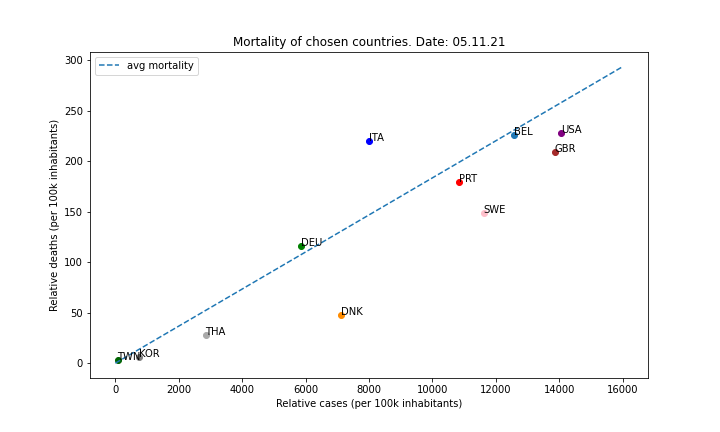
\includegraphics[width=0.8\textwidth]{figures/mortality_plot.png}
    \caption{Relative cases and deaths, giving mortality for each country along with the average mortality.}
    \label{fig:mortality}
\end{figure}

\subsection*{Detailed Analysis: Denmark and Belgium}

As a first analysis, we want to exemplify how countries that are socioeconomically and geographically very similar can react differently to the circumstances, and thereby manage
the pandemic reasonably well, or not. To this end, we inspect COVID-19 related mortality in the countries of interest. We calculate relative cases as the cumulative number of cases per 100 000 inhabitants,
and likewise relative deaths as the cumulative number of deaths per 100 000 inhabitants. The ratio of the two gives the mortality $m$ per country as
\begin{equation}
    m_c = \frac{\text{cumulative deaths}}{\text{cumulative cases}}
\end{equation}

Figure \ref{fig:mortality} shows the mortality of chosen countries, along with the average mortality as the mean $m = \frac{\sum_c^C m_c}{C}$ where $C$ is the number of countries. Here, one can clearly see
that countries drastically differ in relative cases and relative deaths. Asian countries like Taiwan, Thailand or South Korea show significantly less relative cases and relative deaths, meaning they were able to actively control the spread of the virus in their countries thoughout the pandemic. Mortality still goes along the average, since the average mortality is a property of the disease initiated by the virus itself. On the other hand Denmark, for example, has
a very low mortality below the average, which raises the question why that is, since Denmark also has a comparable number of cases to Germany, Austria or Italy.
To study this effect, we choose Denmark and one other country and compare their countermeasures
and testing policies. The most suitable candidates for a comparison to Denmark from figure \ref{fig:mortality} are Germany, Austria or Italy. However, they do not provide sufficient data on testing and policies for an appropriate comparison. Many non-European countries are difficult because of a great gap in socioeconomic factors for most countries, which is shown to influence
the course of an epidemic \cite{mena2021socioeconomic, bennett2021all}. For this reason, Belgium is chosen as a candidate. Although there
are much more cases in Belgium, there are a number of reasons the countries are interesting to compare. First, they are geographically very similar. Both are central-European countries that share land borders with other countries, where the cross-country movement is higher than e.g. on islands. Second, they are very compararble when it comes to socioeconomics: Belgium and Denmark approximately have the same GDP per capita (although slightly higher in Denmark), the median age nearly the same and the share of older and thus more vulnerable people is similar (slightly more people older than 70 in Belgium). Figure \ref{fig:socio_bel_den} compares GDP, median age, age groups and poverty rates of the two countries along with Germany as a reference. And third, the two countries applied drastically different testing strategies and other measures and the gap in mortality is very large, thus interesting to compare.

\begin{figure}[htb]
    \centering
    \includegraphics[width=\textwidth]{figures/Socioeconomic_bel_dnk.png}
    \caption{Comparison of GDP per capita, age groups and extreme poverty rate in Belgium, Denmark and Germany for comparison (missing Germany data for poverty).}
    \label{fig:socio_bel_den}
\end{figure}




\begin{figure}[htb]
    \centering
    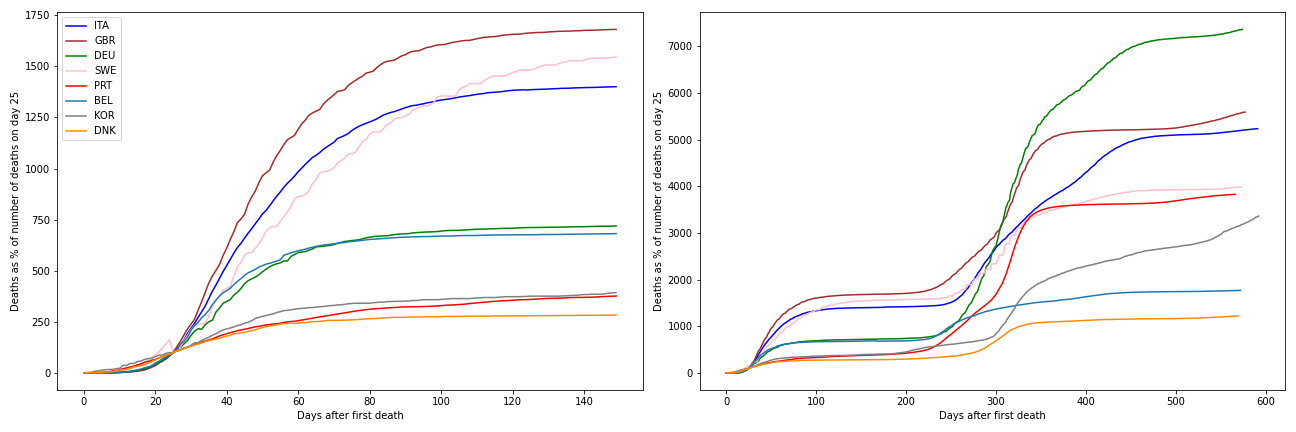
\includegraphics[width=\textwidth]{figures/deaths_combined_2plot.png}
    \caption{Result of Middelburg and Rosendaal's method \cite{middelburg2020covid}. Left: firt wave (up to 150 days). Right: Complete time frame. Included are Italy, Germany, Belgium Denmark, Portugal, Great Britain and Korea. The USA is not included here because the value is significantly larger than all others, reaching up to 45 000 and rendering all other curves incomparable.}
    \label{fig:deaths_all}
\end{figure}

Having selected Belgium and Denmark as our candidates, we apply the method for cross-country comparisons as presented by
Middelburg and Rosendaal. First, they argue that comparison of relative deaths gives a more stable metric rather than relative
cases \cite{middelburg2020covid}, additionally it reduces the impact of testing strategies. Second, they propose to eliminate the exact date in the comparison and to create \textit{index} dates for each country. The index date refers to the day of the first recorded death. This procedure eliminates the difference
in time when the pandemic reaches each country. The time dimension throughout the pandemic is then expressed as \textit{days after first recorded death}. Subsequently, they present a stable expression of the number of deaths per country. Instead of looking at deaths per 100 000 inhabitants, they select a specific date, that is day 25 after the index date, and express future deaths
as a percentage of the number of deaths on day 25 after the index date \cite{middelburg2020covid}.
The results of this method for chosen countries can be seen in figure \ref{fig:deaths_all}.
This setup shows interesting and unintuitive results. It shows that Italy handled the
second wave of infections reasonably better than Germany, as the curve of Germany surpasses the Italian at the beginning of the second wave. The method also confirms
what was already prominent in figure \ref{fig:mortality}: Belgium has a number of deaths (as percentage) approximately twice as high as Denmark after the first wave of infections. After the second wave, Belgium still shows higher numbers than Denmark, but less than before.
Although both waves of infections also hit Denmark around the same time, the curve flattens very early, before the exponential growth becomes too dominant to contain widespread distribution of the virus. They effectively managed to break the wave, and the reasons for this will be analysed.

The two most obvious explanations for the discrepancy of deaths between Belgium and Denmark are 1) more stringent policies and measures in Denmark that helped to reduce transmission of the virus and thus also deaths and 2) differences in testing strategies,
as more testing allows early identification of infected people and thus interrupts transmission chains before they reach 
vulnerable people that are likely to die from an infection.
Both points can be analyzed, as the OWID dataset provides metrics for both testing and stringency.

\begin{figure}[htb]
    \centering
    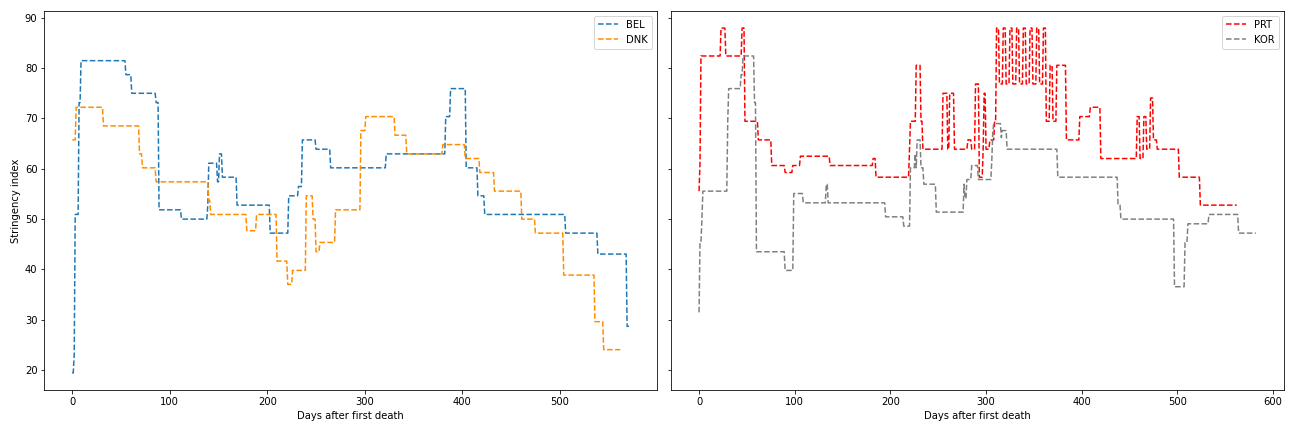
\includegraphics[width=\textwidth]{figures/stringency_2plot.png}
    \caption{Oxford Stringency Index \cite{hale2021global} in Belgium, Denmark (left) and Portugal, Korea (right).}
    \label{fig:stringency}
\end{figure}

We first attend to the stringency of policies. The OWID dataset contains the \textit{Oxford Stringency Index (OSI)}, as a part of the 
University of Oxford's Government Response Tracker \cite{hale2021global}. The stringency index ranges from 0 to 100 and brings together multiple 
measurements of 'severeness' of lockdown measures and other restrictions that affect everyday-life of people, such as
school and workplace closures, cancellation of public events, restrictions on movement and gathering size, closure of public transportation, and others. Overall the OSI allows to assess how strict lockdown measures are in countries and thus 
to compare them.
Figure \ref{fig:stringency} compares the OSI of Belgium and Denmark throughout the pandemic. There is no drastic difference in stringency,
at some points, Belgium employed even stricter measures than Denmark, which can not explain the substantial difference in 
case and death numbers between the countries.



Next we assess the testing strategies of the countries.
The ratio \textit{tests per case} as well as the \textit{positive rate} will be compared to assess the difference in testing. Figures \ref{fig:testing_bel_den} presents the result for Belgium and Denmark, while sill adopting the 
method using index dates instead of calendar dates as presented in \cite{middelburg2020covid}. Here one can clearly see the difference in testing strategies. Throughout the pandemic, Belgium only tested more when case numbers are already rising again, leading to a high positive rate. According to the WHO \cite{world2020public}, a positive rate below 5\% is an indicator that an epidemic is under control in a country. Belgium rarely reaches below this threshold, while at other points reaching positive rates up to 20\%. This means that too few tests were made throughout the pandemic. Denmark, on the other hand, shows a positive rate which rarely reaches 5\% (only after day 500, when already more than 50\% of people were vaccinated), meaning that, by intensive testing, they were able to contain the epidemic and keep death numbers low.

\begin{figure}[htb]
    \centering
    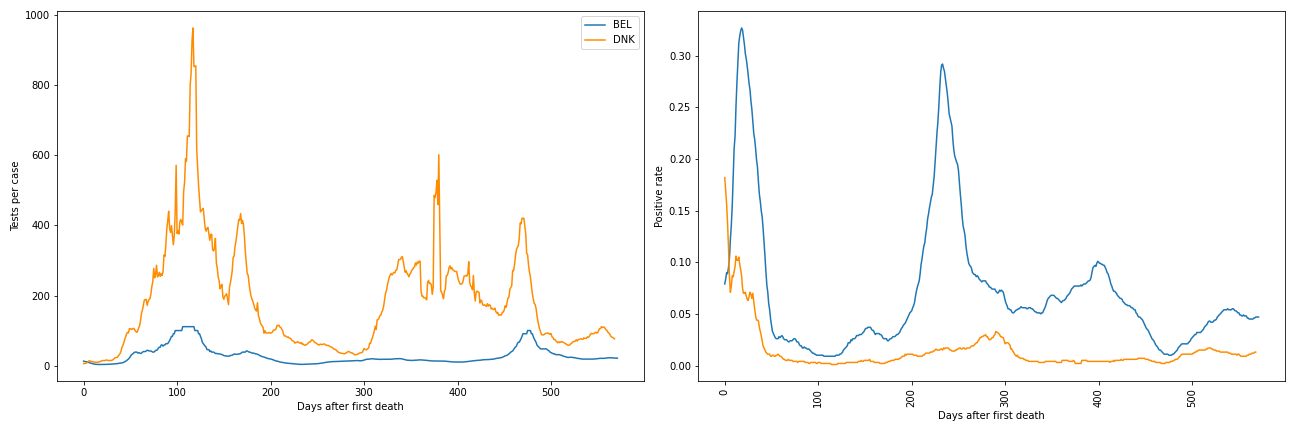
\includegraphics[width=\textwidth]{figures/testing_bel_dnk.png}
    \caption{Testing strategies in Belgium and Denmark.}
    \label{fig:testing_bel_den}
\end{figure}

\begin{figure}[htb]
    \centering
    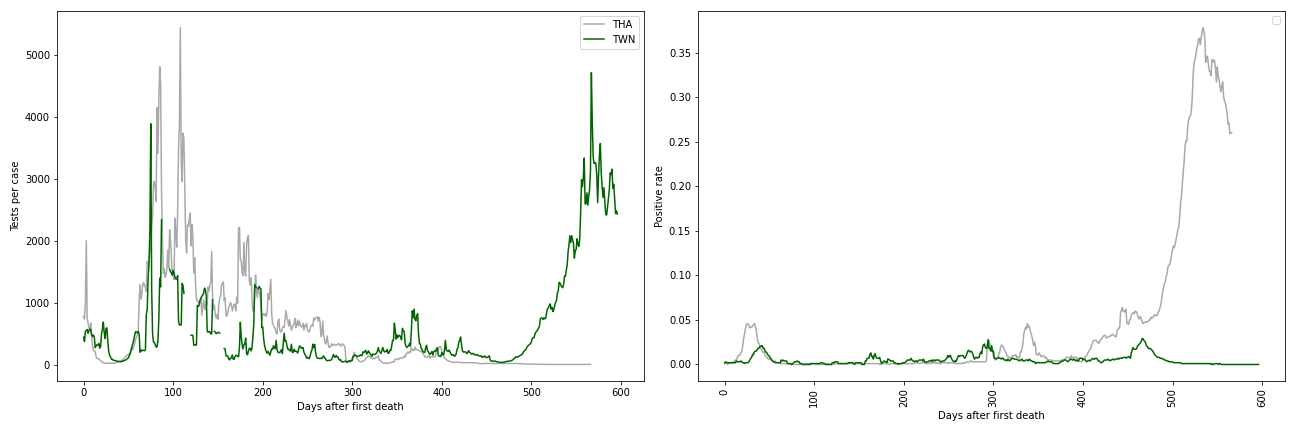
\includegraphics[width=\textwidth]{figures/testing_tha_twn.png}
    \caption{Testing strategies in Thailand and Taiwan.}
    \label{fig:testing_tha_twn}
\end{figure}

This is a confirmation that testing is extremely important, and that the positive rate is an appropriate factor to consider, along with the widely used incidence. An even more extreme example for this can be seen in Asian countries, namely Taiwan and Thailand. Figure \ref{fig:testing_tha_twn} shows the testing strategies of the countries, and we can see that the positive rate remained extremely low (Apart from day 500 when positive rate is exploding in Thailand. The reason for this behaviour is not clear, but probably attributed to continuing vaccination programs.). This gives a good explanation on why these countries handled the pandemic so well and were able to keep death numbers so low. Figure \ref{fig:deaths_pos_rate} shows the course of the pandemic with deaths and positive rate for a number of countries. One can observe that a substantial rise in death numbers always correlates with a spark in positive rate. This is again support for the importance of the positive rate as an epidemiological factor to consider.


\begin{figure}[htb]
    \centering
    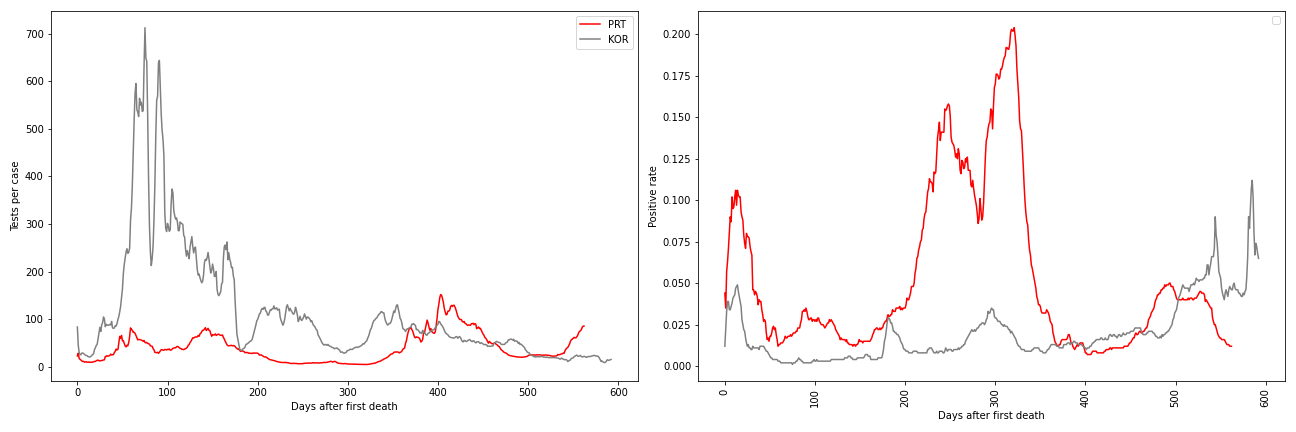
\includegraphics[width=\textwidth]{figures/testing_prt_kor.png}
    \caption{Testing numbers in Portugal and Korea.}
    \label{fig:prt_kor}
\end{figure}

\begin{figure}[htb]
    \centering
    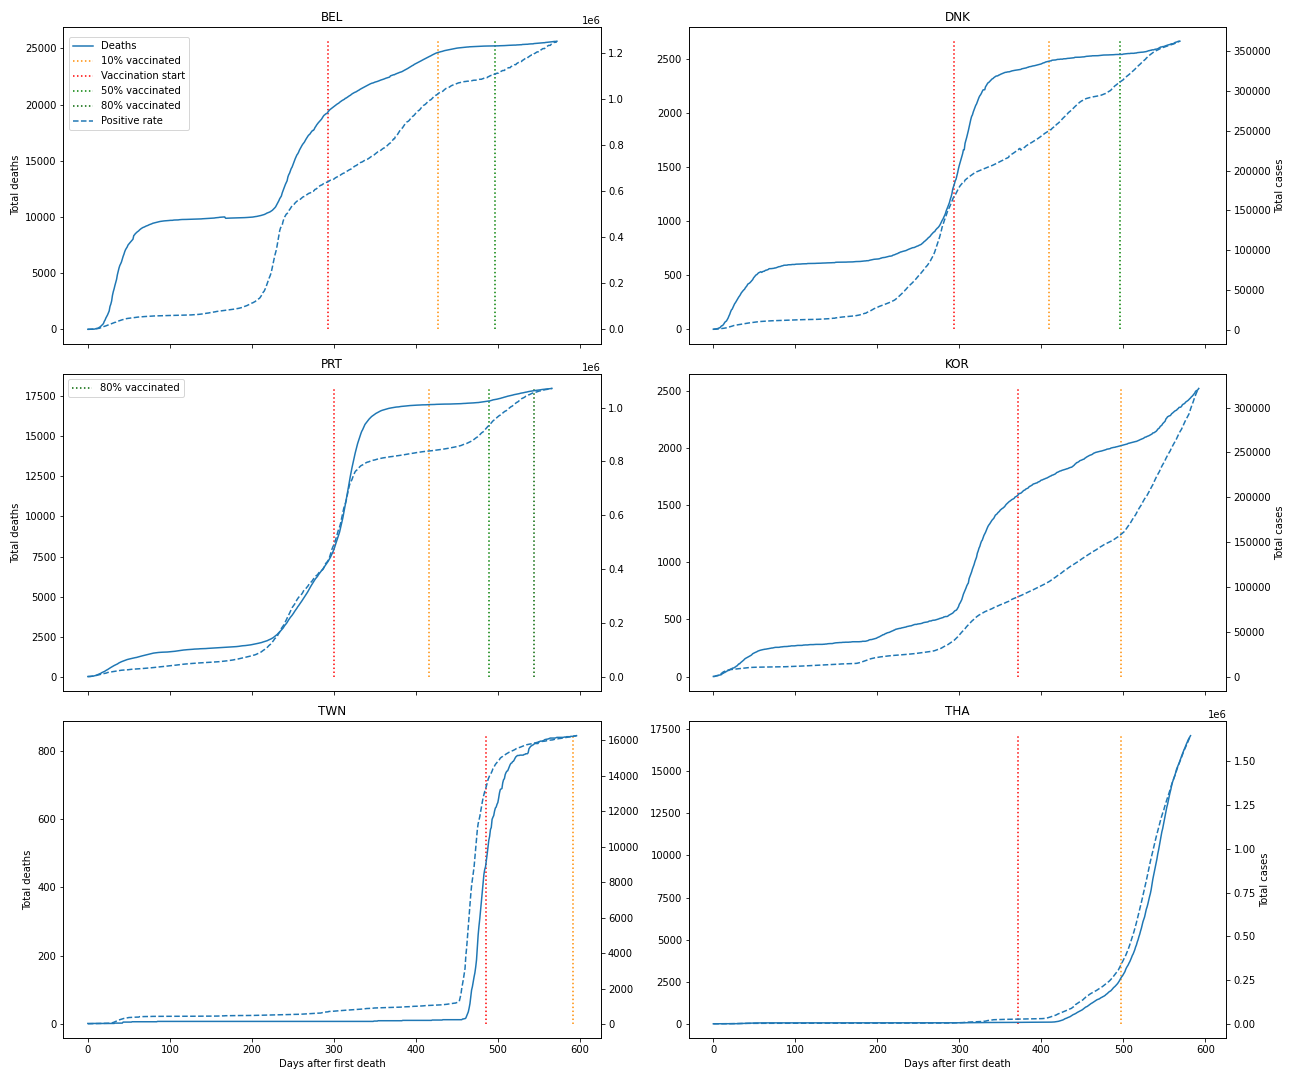
\includegraphics[width=\textwidth]{figures/deaths_cases_6.png}
    \caption{Cumulative (total) deaths and cumulative cases per country, along with vaccination milestone marks. For all countries (except Korea) deaths increase less when highly vulnerable people are vaccinated, while case numbers still rise. Note that -- opposite to other plots -- we look at the \textit{total} deaths here, not as a percentage of deaths on day 25.}
    \label{fig:cases_deaths_all}
\end{figure}

We saw that testing strategies drastically influence the number of COVID-related deaths in Belgium and Denmark. Now, it will be investigated if the importance of testing remains when a reasonably large share of the population are vaccinated, and how vaccinations relate to death numbers.
To this end, Portugal and Korea are chosen as candidates for a direct comparison. Figure \ref{fig:prt_kor} shows testing numbers for the two countries. We can see that, from approximately day 400 onward, testing numbers are very similar, ruling out the effect of different testing strategies on death numbers, like it was showed in the first part. Figure \ref{fig:deaths_all} and also figure \ref{fig:cases_deaths_all} show that the number in Korea deaths still increase approximately at the same level than before, while in Portugal, where more than 50\% of the population is vaccinated, deaths significantly decline. Even when cases begin to rise around day 480, the increase of deaths remains low. We can see a similar behaviour for Denmark and Belgium in figure \ref{fig:cases_deaths_all}, while in Thailand deaths were rising exponentially, as they seem to have quit their testing strategies. Taiwan was able to break the exponential growth very early, again by massive testing, as we can see by their testing numbers at that time in figure \ref{fig:testing_tha_twn}.

The observation can be regarded as support for the claim that vaccinations drastically influence the pandemic situation when a large share of the population is vaccinated. If that is the case, testing strategies as the main factor of the epidemic situation are ruled out. However, when there are not enough people vaccinated, testing still remains the most important measure, as one can see from the example of Taiwan and Thailand. Admittedly, seasonal effects are not considered here.


\begin{figure}[htb]
    \centering
    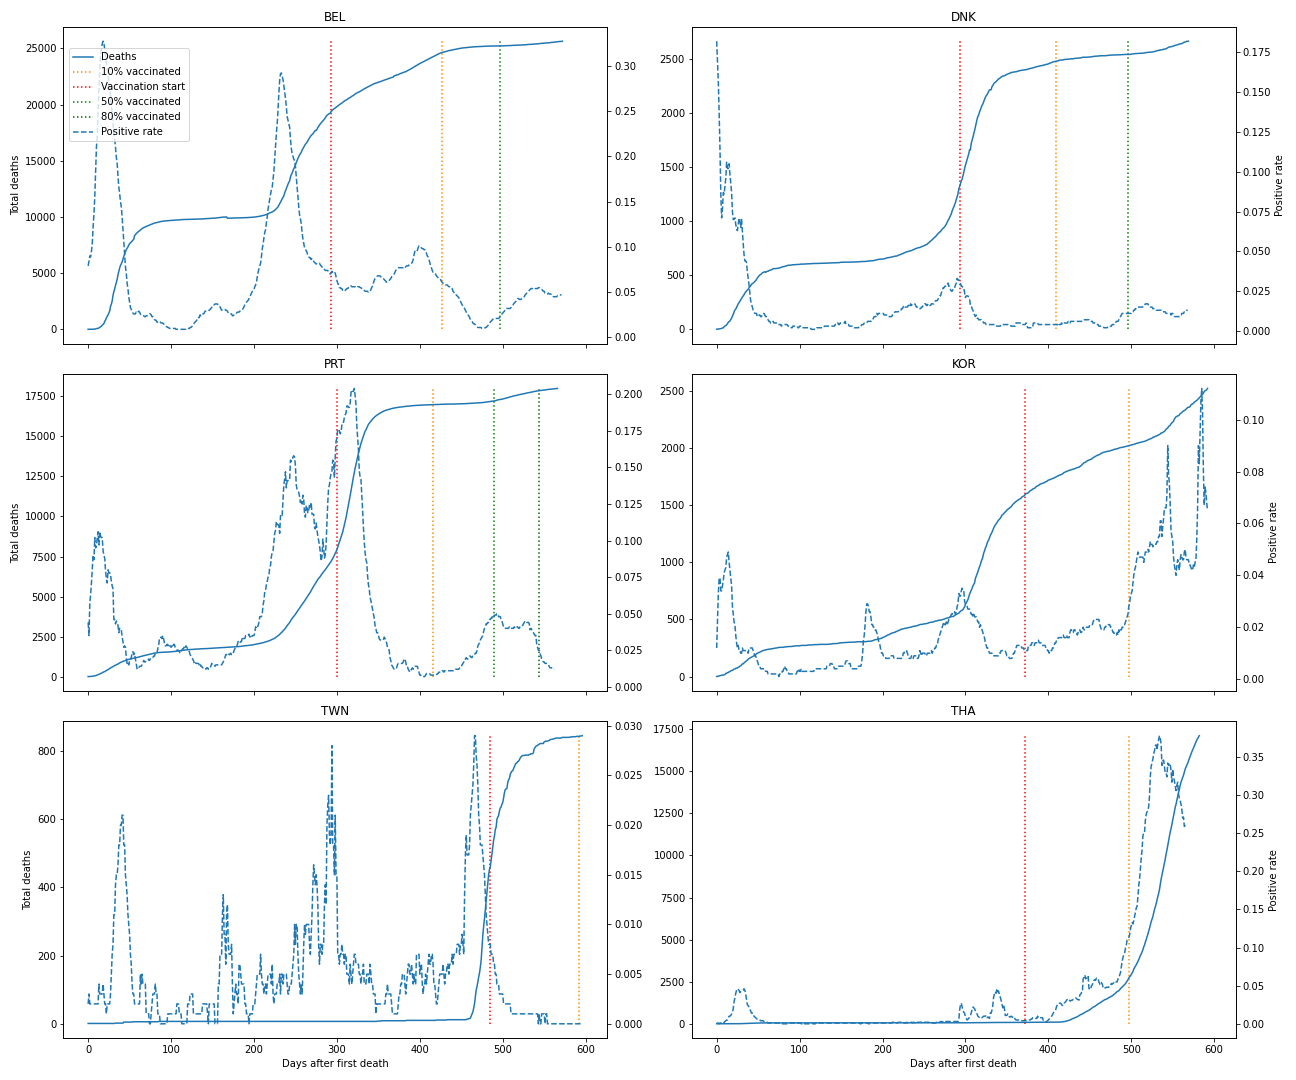
\includegraphics[width=\textwidth]{figures/deaths_posrate_6.png}
    \caption{Cumulative (total) deaths and positive rate per country, along with vaccination milestone marks. }
    \label{fig:deaths_pos_rate}
\end{figure}


\section{Limitations}
Although all work has been conducted to my best knowledge, I am no expert in epidemiology, and all results have to be considered with care. It is not the intention here to gain new significant scientific results but to provide more empiric evidence for mostly already known facts.
Accounting for all epidemiological factors here is out of scope. For example, during the course of the pandemic, the virus of interest that dominated the pandemic situation changed, from the alpha variant, to beta and now delta. Each of the variants has different properties and the epidemiological situation changed from time to time. This factor has not been considered. Seasonal effects also remain mainly unconsidered since it is difficult to include this factor without the use of sophisticated models. Seasonal effects heavily influence the spread of the virus, and it is difficult to attribute the significant drop in case numbers in spring 2021 to the higher temperatures in summer or to the progress in vaccination programs.

\section{Conclusion and Future Work}

The present work presented a data-analytic view on the COVID-19 pandemic, with regards to testing strategies and vaccination programs. An epidemiological framework was applied to provide an appropriate comparison of the pandemic situation in different countries, which accounts for distorting variables \cite{middelburg2020covid}. Subsequently, a detailed comparison between Denmark and Belgium as contenders of two very different strategies during the pandemic, was conducted, which supports the claim that testing remains an important factor to control an epidemic and avoid lockdowns. The positive rate was shown to be a good indicator of the situation in a country. If positive rates are too high, the control over the epidemic tends to be lost. Thus, the positive rate should be considered along with the case incidence. Vaccination progream heavily influence the pandemic situation, as we have seen from the comparison of Portugal, Korea and also Denmark and Belgium. However, a large share of the population has to be vaccinated in order to quit extensive testing without losing control over the pandemic. The example of Thailand showed this behaviour, while Taiwan held on to testing and was able to break a wave very early on.

The work enqueues in a long list of COVID-related data analysis projects and can be seen as additional support for (mostly) known epidemiological facts. Future work could include applying sophisticated models to account for seasonal effects and other factors that were out of scope for this factor. Lastly, future data will show how the situation changes if vaccinations lose their effect on preventing serious courses of disease, which is a current discussion and an interesting topic to study.

\newpage

\printbibliography
\end{document}
